\documentclass[12pt, oneside]{article}
\usepackage{geometry}                		% See geometry.pdf to learn the layout options. There are lots.
\geometry{letterpaper} 
\usepackage{amsmath}
\usepackage{amsthm}
\usepackage{amssymb}
\usepackage{graphicx}
\usepackage{color}
\usepackage{float}
\usepackage{subfig}
\usepackage[flushleft]{threeparttable}
\usepackage{gensymb}
\usepackage{multirow}
\usepackage[dvipsnames]{xcolor}
\newcommand{\BibTeX}{\textsc{Bib}\TeX}
%opening
\title{Instructions for running DNS code and plotting results}
\author{}

\begin{document}
\maketitle
\tableofcontents

\newpage

\section{DNSMST setup}

\begin{figure}[H]
  \begin{center}
  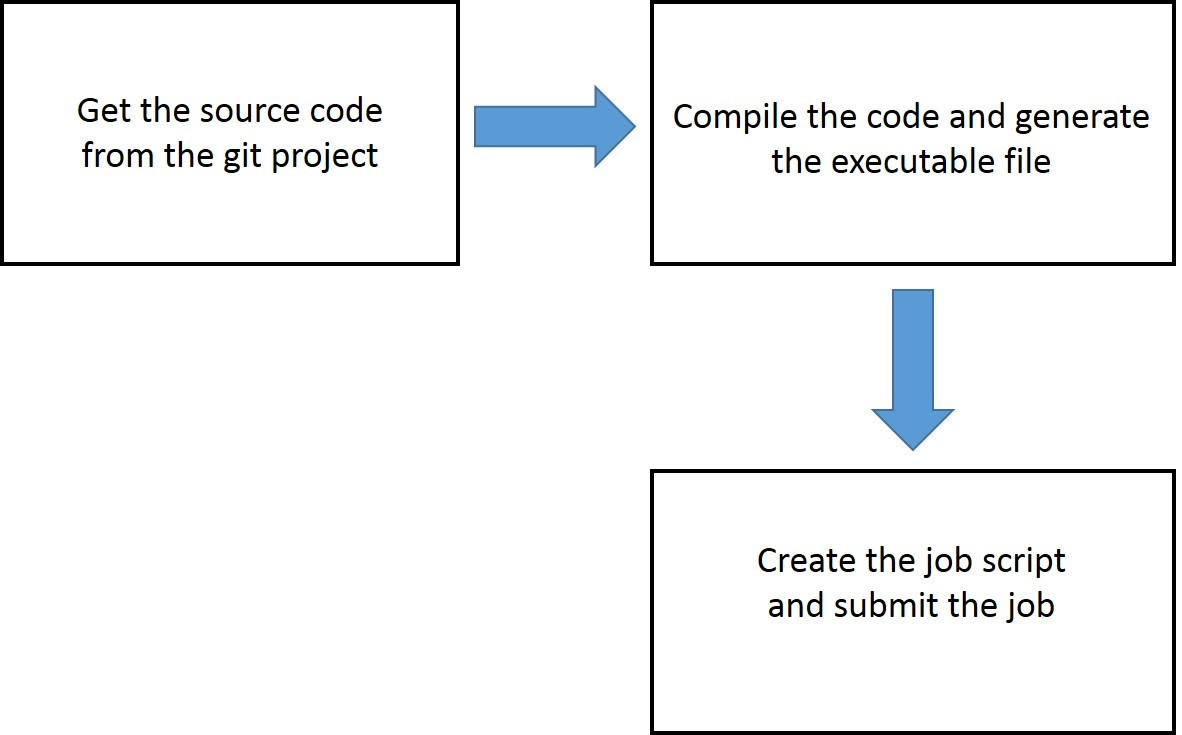
\includegraphics[width=0.6\textwidth]{FIGS/DNSMST.png}
  \caption{The procedures for using DNSMST.}
  \label{fig:BCGrid}
  \end{center}
\end{figure}

\subsection{Getting the source code}

Type the following command to get the DNS source code from the git project.

\begin{verbatim}
$ git clone git@git.mst.edu:duanl/DNSMST_HDF5.git
\end{verbatim}

\subsection{Compiling the source code}

The following example will show how to compile the source code using cmake system.

\begin{verbatim}
~~~~~~~~~~~~~~~~~~~~~~~~~~~~~~~~~~~~~~
! In the folder DNSMST_HDF5
$ mkdir build
$ cd build
$ FC=mpif90 cmake ..   !(this line is for Nic)
$ FC=ftn cmake ..      !(this line is for BlueWaters)
$ make
~~~~~~~~~~~~~~~~~~~~~~~~~~~~~~~~~~~~~~
\end{verbatim}

Please remember to change the value of the variables "imax, jmax, kmax, inode, jnode" in the file "src/modules/modHead.f90" before compiling the source code. Please delete all the files in the folder "build" when you try to re-compile the code.

\subsubsection{HPC: Nic}

Before compiling the source code, the environment should be changed.

In the file ".bashrc", please add the following commands:

\begin{verbatim}
~~~~~~~~~~~~~~~~~~~~~~~~~~~~~~~~~~~~~~
module load phdf5/i12
module load intel/intel-12
module load openmpi/intel-12
module load fftw-3.3.4
. /share/duan/tools/src/hdf5_env
. /share/duan/tools/src/cmake_env
~~~~~~~~~~~~~~~~~~~~~~~~~~~~~~~~~~~~~~
\end{verbatim}

After saving the file ".bashrc", please type the following command:
\begin{verbatim}
$ source ~/.bashrc
\end{verbatim}




\subsubsection{HPC: BlueWaters}

In the file ``.bashrc``, please add the following commands:

\begin{verbatim}
~~~~~~~~~~~~~~~~~~~~~~~~~~~~~~~~~~~~~~
export NO_DYNAMIC=1
module load cmake/3.1.3
module load cray-hdf5-parallel/1.8.16
~~~~~~~~~~~~~~~~~~~~~~~~~~~~~~~~~~~~~~
\end{verbatim}

After saving the file ".bashrc", please type the following command:
\begin{verbatim}
$ source ~/.bashrc
\end{verbatim}
\subsection{Setting up the run folder}
Create a folder for your run.

\noindent In this folder copy the curvdns and deck3d.inp file and  make 2 folders:

\indent 1st a folder for flow initialization, I reccomend calling it InitDNS
        
\indent 2nd a folder called REST, this folder \textbf{MUST} be named this and in caps


\noindent At this point your folder should look like this.

\begin{figure}[H]
  \begin{center}
  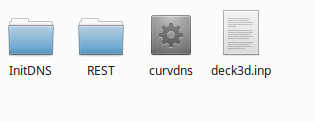
\includegraphics[width=0.6\textwidth]{FIGS/Folder_setup.png}
  \caption{Work Folder.}
  \label{fig:BCGrid}
  \end{center}
\end{figure}


\noindent Compile and copy blinit and blinit.inp into the InitDNS folder. 
\begin{verbatim}
 blinit is located in: 
 dnsmst_utilities/src/serial/Initialization/Init_wave/InitP3d/
 You can compile the code with the make command
\end{verbatim}
\noindent Add the flow initialization file to the InitDNS folder

\noindent Edit the .inp file for your case. 

\noindent The common things to change will be: imax/ibeg, kmax/iend, kend and flowfilename.
\indent iend-ibeg+1 should be equal to your domain size in the i direction

\indent kend should be the domain size in the k direction

\indent flowfilename should be the location of your flow initialization file

\noindent Now request an interactive job:
\begin{verbatim}
 You can use the command 
 qsub -I -V -l nodes=1:ppn=4 -l walltime=1:00:00 -q @nic-cluster.mst.edu 
 to do this.
 For a more complete explination of this look the git project Wiki:
 git@git.mst.edu:czb58/HPC_User_Guide.git
\end{verbatim}

\noindent navagiate to and run the blinit code with the command:
\begin{verbatim}
 ./blinit < blinit.inp
\end{verbatim}


\noindent Copy or link the flowdata and grid file into REST

\noindent In the REST file make a copy or link of the flowdata file and rename it baseflow.h5




\subsection{Running the executable file}

Check the detail information on the git project Wiki: 
\begin{verbatim}
 git@git.mst.edu:czb58/HPC_User_Guide.git
\end{verbatim}






\section{DNSMST utilities setup}

\subsection{Getting the source code}

Type the following command to get the source code from the git project.

\begin{verbatim}
git clone git@git.mst.edu:czb58/dnsmst_utilities.git
\end{verbatim}

\subsection{Compiling the source code}
Move to the folder of the tool you want to use HEAD at the branch. Loc
Postprocessing tools are located at /src/parallel/Postprocessing/ or /src/serial/Postprocessing/
Inside of the folder of the tool you want to use the command 'make', this will compile the code inside the folder

\subsection{Running the executable file}
Create a folder in the folder used in section 1.3

Copy the executable and the .inp file to this folder

Edit the .inp file:
	include the path to flow data, in this case it should be ../REST/
	Set the i,j,k max values, these correspond to the i,j,k values used in DNSMST
	Alter any program specfic values

Request an interactive job, examples are shown in section 5 of the wiki
	For simple cases make sure the number of requested processors are low, do this by altering the value after ppn= this sets how many processors are requested

When your job has started navagiate to the folder the desired tool was put in, the folder from section 2.2

Type the following command 
\begin{verbatim}
./executable < file.inp
\end{verbatim}
	where executable is the name of what you want to use and file.inp is the .inp file.
	This is saying to read the file.inp into the executable and run it









Generate the initial grid and flowdata. The grid and flowdata file should be put in the folder "REST". The file baseflow.h5 is a copy of flowdata\_00000000.h5
\begin{verbatim}
 dnsmst_utilities/src/serial/Initialization/Init_wave/InitP3d/
\end{verbatim}

\noindent
Calculate the grow factor.
\begin{verbatim}
 dnsmst_utilities/src/serial/Initialization/Init_wave/CalGrowth/
\end{verbatim}


\noindent
Calculate the Fourier mode.
\begin{verbatim}
dnsmst_utilities/src/serial/Postprocessing/Fourier/
\end{verbatim}


\section{Plot}

Type the following command to open tecplot 360.

\begin{verbatim}
$ tec360 
\end{verbatim}



\section{Useful commands}

\subsection{Basic Vim commands}
\begin{verbatim}
https://coderwall.com/p/adv71w/basic-vim-commands-for-getting-started
\end{verbatim}

\subsection{Version Control with Git}
\begin{verbatim}
https://swcarpentry.github.io/git-novice/
\end{verbatim}

For each new computer, add the ''SSH Keys'' to your git profile.

Your ''SSH Keys'' are located in AvatarIcon/Settings/SSH Keys 

\begin{verbatim}
 settings -> SSH Keys
\end{verbatim}
\begin{verbatim}
 Your SSH Key should be in the file ``~/.ssh/id_rsa.pub''. 
 If you don't have this file, please generate it using the ssh-keygen command.
\end{verbatim}




\subsection{Basic Linux Commands}
\begin{verbatim}
http://www.comptechdoc.org/os/linux/usersguide/linux_ugbasics.html
\end{verbatim}


\subsection{HPC User Guide}

Goto the following project, the 'Wiki' page shows how to use different HPCs.

 \begin{verbatim}
git@git.mst.edu:czb58/HPC_User_Guide.git
 \end{verbatim}
 

\subsection{Modules on Nic}

Please put the following modules in the file '.bashrc'. The file can be opened as
\begin{verbatim}
vi ~/.bashrc 
\end{verbatim}
\begin{verbatim}
module load phdf5/i12
module load openmpi/intel-12
module load fftw-3.3.4
\end{verbatim}
  
  
% 
% \bibliography{conf_M14}
% \bibliographystyle{aiaa}
% 

\end{document}
